\section{Model-based Testing}\label{sec:model_based_testing}

Model-based testing is a testing technique where a System Under Test (SUT) is tested for conformance to a model description of the system. The general setup for this process is depicted as a UML sequence diagram in Figure~\ref{fig:model_based_testing}. The specification of a system is provided as a model to a test derivation component which generates a test suite. The test suite is used by a test execution component to test the SUT. Tests are executed by providing input/stimuli to the SUT and monitoring the output/response. The test execution component evaluates whether the correct responses are given. It gives a 'pass' or 'fail' verdict depending on whether the SUT conforms to the model or not.

\begin{figure}[ht]
  \begin{center}
    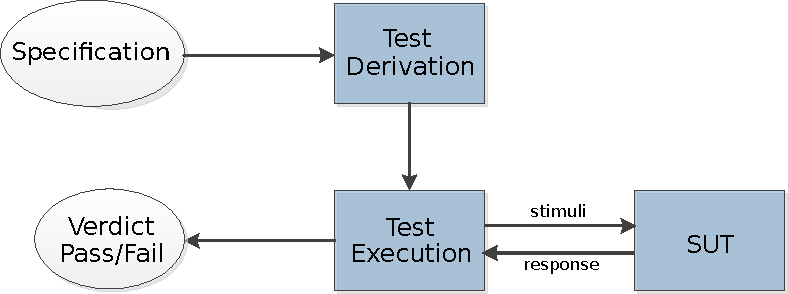
\includegraphics[width=0.6\textwidth]{model-based-testing.pdf}
  \end{center}
  \caption{A general model-based testing setup}
  \label{fig:model_based_testing}
\end{figure}

This type of model-based testing is called \textit{batch testing} or \textit{offline testing}. Another type of model-based testing is \textit{on-the-fly} testing. The main difference is that no test cases are derived, instead a transition in the model is chosen and tested on the system directly. The general architecture for this process is shown in Figure~\ref{fig:model_based_testing_on_the_fly}. An example of an on-the-fly testing tool is TorX~\cite{Tretmans:TorX}.

\begin{figure}[ht]
  \begin{center}
    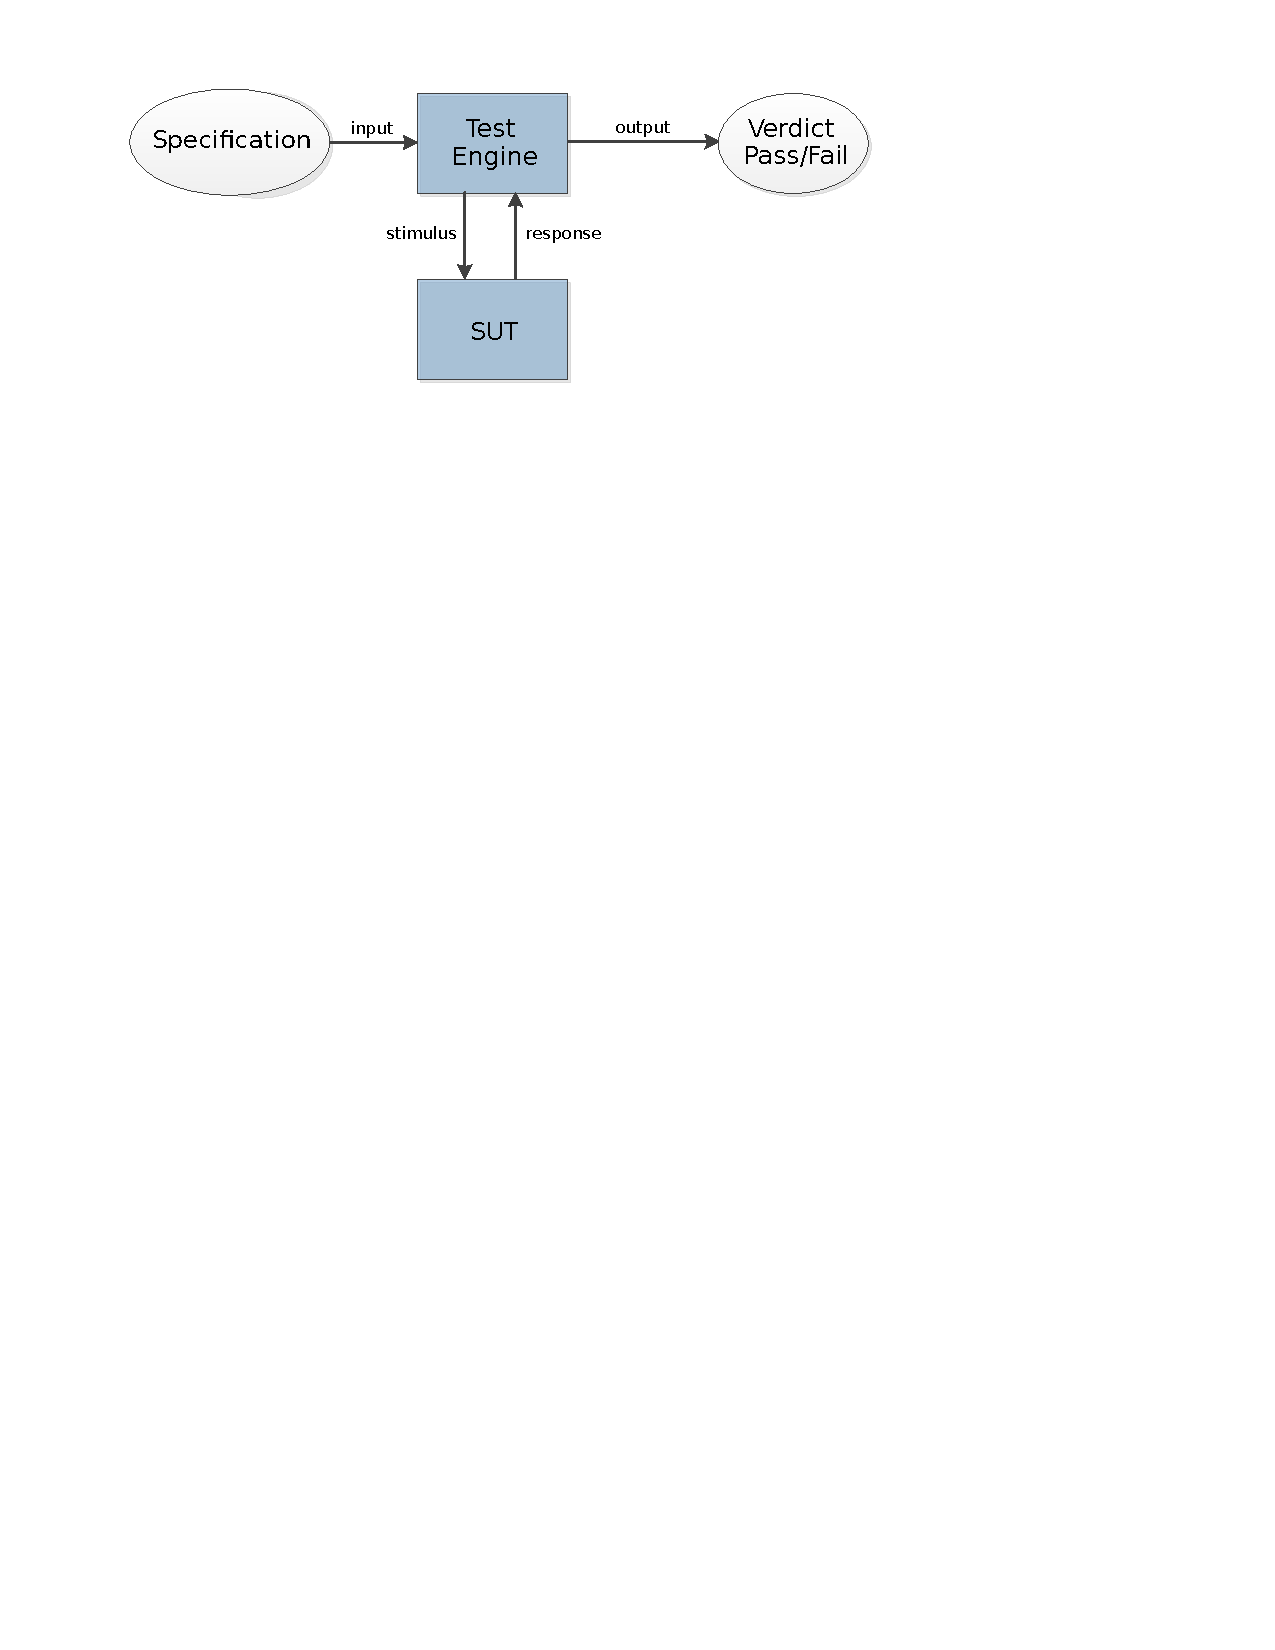
\includegraphics[width=0.6\textwidth]{mbt-on-the-fly.pdf}
  \end{center}
  \caption{A general 'on-the-fly' model-based testing setup}
  \label{fig:model_based_testing_on_the_fly}
\end{figure}

Variations of state machines and transition systems have been widely used as the underlying model for test generation. Other tools use the structure of data types to generate test data. 

The stucture of the rest of this section is as follows. First, previous work on model-based testing is given. Then, Labelled Transition Systems are introduced. This is a basic formalism useful to understand the models in the rest of the paper, namely Graph Grammars and Symbolic Transition Systems. Next, an adaptation of Labelled Transition Systems, the Input-Output Transition System is described. This is a useful formalism for Model-Based Testing. Finally, the notion of \textit{coverage} is explained.

\subsection{Previous work}
Transition-based formal testing theory was introduced by De Nicola et al.~\cite{denicola:testing}. The input-output behavior of processes is investigated by series of tests. Two processes are considered equivalent if they pass exactly the same set of tests. This testing theory was first used in algorithms for automatic test generation by Brinksma~\cite{brinksma:testgeneration}. This led to the so-called \textit{canonical tester} theory. Tretmans gives a formal approach to protocol conformance testing (whether a protocol conforms to its specifications) in~\cite{Tretmans:conformancetesting} and an algorithm for deriving a sound and exhaustive test suite from a specification in~\cite{Tretmans:testgeneration}. A good overview of model-based testing theory and past research is given in "Model-Based Testing of Reactive Systems"~\cite{Broy:ModelBasedTesting}.

\subsection{Labelled Transition Systems}
A Labelled Transition System (LTS) is a structure consisting of states with labelled transitions between them.
\vspace{10px}
\begin{definition} Labelled Transition Systems \\
An LTS is a 4-tuple	$\langle \States, \Labels, \Transitions, \initialState\rangle$, where:
\begin{itemize}
\item $\States$ \newnot{symbol:States} is a finite, non-empty set of states
\item $\Labels$ \newnot{symbol:Labels} is a finite set of labels
\item \newnot{symbol:Transitions} $\Transitions \subseteq \States \times (\Labels \cup \{\tau\}) \times \States$, with $\tau \notin \Labels$, is the transition relation
\item \newnot{symbol:initialState} $\initialState \in \States$ is the initial state.
\end{itemize}
We write $\state \xrightarrow{\mu}\state'$ if there is a transition labelled $\mu$ from state $\state$ to state $\state'$, i.e., $(\state, \mu, \state') \in \Transitions$. $\state, \state'$ are called the source and target states of the transition respectively. The informal idea of such a transition is that when the transition system is in state $\state$ it may perform action $\mu$, and go to state $\state'$.
\end{definition}

\paragraph*{Input-Output Transition Systems}
A useful type of transition system for model-based testing is the Input-Output Transition System (IOTS) by Tretmans~\cite{Tretmans:testgeneration}. Assuming that implementations communicate with their environment via inputs and outputs, this formalism is useful for describing system behavior. The system is regarded as a black box and the IOTS specifies the allowed inputs and outputs.

IOTSs have the same definition as LTSs with one addition: each label $\ltsLabel \in \Labels$ has a type $\iotype \in \IOTypes$, where $\IOTypes = \{input, output\}$\newnot{symbol:IOTypes}. Each label can therefore specify whether the action represented by the label is a possible input or an expected output of the system under test. An IOTS is formally defined as:
\vspace{10px}
\begin{definition} Input-Output Transition Systems \\
An IOTS is a 4-tuple $\langle \States, \Labels, \IOTransitions, \initialState\rangle$\newnot{symbol:IOTransitions}, where $\IOTransitions \subseteq \Transitions \times \IOTypes$ are the input-output transitions.
\end{definition}
\vspace{10px}
When the transition system is in the source state of an input transition, the input can be given to the SUT. When the transition system is in the source state of an output transition, the output should be observed from the SUT. In both cases, the transition system advances to the target state of the transition. The case where a state has both input and output transitions is not considered in this report.

An example of such an IOTS is shown in Figure~\ref{fig:iots_example}. This system allows an input of 20 or 50 cents and then outputs tea or coffee accordingly. The inputs are preceded by a `?', the outputs are preceded by an `!'. This system is a specification of a coffee machine. A test case can also be described by an IOTS with special pass and fail states. 

A test case for the coffee machine is given in Figure~\ref{fig:iots_test}. The test case shows that when an input of `50c' is given, an output of `coffee' is expected from the tested system, as this results in a `pass' verdict. When the system responds with `tea', the test case results in a `fail' verdict. The pass and fail verdicts are two special states in the test case, which are sink states, i.e., once in either of those the test case cannot leave that state. 

Test cases should always reach a pass or fail state within finite time. This requirement ensures that the testing process halts.
\begin{figure}[ht]
  \begin{center}
    \subfloat[An IOTS]{\label{fig:iots_example}$\xymatrix{
    \bullet \ar[r]^{?50c} \ar[d]_{?20c} & \bullet \ar[d]^{\mathit{!coffee}} \\
    \bullet \ar[r]_{!tea}       & \bullet }$
}
    \subfloat[An IOTS test case]{\label{fig:iots_test}$\xymatrix{
    \bullet \ar[r]^{!50c} & \bullet \ar[r]^{\mathit{?coffee}} \ar[d]_{?tea} & {pass}\\
    & {fail}}$}
  \end{center}
  \caption{The specification of a coffee machine and a test case as an IOTS}
\end{figure}

\paragraph*{Coverage}\label{sec:coverage}
The number of tests that can be generated from a model is potentially infinite. Therefore, there must be a test selection strategy to maximize the quality of the tests while minimizing the time spent testing. Coverage statistics help with test selection. Coverage statistics are calculated to indicate how adequately the testing has been performed~\cite{Zhu:coverage}. These statisics are therefore useful metrics for communicating how much of a system is tested.

One type of coverage is \textit{white-box coverage} or \textit{code coverage}: This coverage statistic measures how much of the lines of codes in the implementation is tested. A line of code is considered tested when it is executed during the test run.

When the SUT is a black box, which often is the case, typical coverage metrics for LTSs are \textit{state and transition coverage}~\cite{Lee:testing, Nachmanson:testing, Hasan:testing}. This coverage statistic measures how much of the model is tested. A state in the model is considered tested when the transition system reaches the state during testing. A transition in the model is considered tested when the transition system is in the source state of the transition and either:
\begin{enumerate}
\item the transition is a stimulus and the input represented by the label of the transition is given to the SUT
\item the transition is a response and the output represented by the label of the transition is observed from the SUT
\end{enumerate}

 State coverage can be measured by dividing the tested states by the total states in the model. The same process applies to transition coverage. As an example, the coverage metrics of the IOTS test case example in~\ref{fig:iots_test} are calculated. The test case tests one path through the specification and passes through 3 out of 4 states and 2 out of 4 transitions. The state coverage is therefore 75\% and the transition coverage is 50\%.

 This example shows that the total number of states and transitions in the transition systems has to be known; coverage statistics cannot be measured on an infinitely large LTS, for example.

